\documentclass[aspectratio=169]{beamer}

\usetheme[progressbar=frametitle]{metropolis}
\usepackage{appendixnumberbeamer}

\usepackage{booktabs}
\usepackage[scale=2]{ccicons}

\usepackage{pgfplots}
\usepgfplotslibrary{dateplot}

\usepackage{xspace}
\newcommand{\themename}{\textbf{\textsc{metropolis}}\xspace}

% Custom colors matching the report
\definecolor{primary}{RGB}{41, 128, 185}
\definecolor{secondary}{RGB}{52, 73, 94}
\definecolor{accent}{RGB}{231, 76, 60}
\definecolor{success}{RGB}{39, 174, 96}
\definecolor{warning}{RGB}{241, 196, 15}
\definecolor{codebackground}{RGB}{248, 248, 248}
\definecolor{codeborder}{RGB}{200, 200, 200}
\definecolor{lightgray}{RGB}{245, 245, 245}

\setbeamercolor{palette primary}{bg=primary,fg=white}
\setbeamercolor{palette secondary}{bg=secondary,fg=white}
\setbeamercolor{palette tertiary}{bg=primary,fg=white}
\setbeamercolor{structure}{fg=primary}
\setbeamercolor{title}{fg=primary}
\setbeamercolor{frametitle}{fg=white}
\setbeamercolor{block title}{bg=primary,fg=white}
\setbeamercolor{block body}{bg=primary!10}
\setbeamercolor{item}{fg=primary}

\usepackage{pdfpages}
\setbeamercolor{section title}{fg=primary,bg=primary}
\setbeamercolor*{structure}{bg=primary!20,fg=primary}
\setbeamercolor*{palette primary}{use=structure,fg=white,bg=structure.fg}
\setbeamercolor{progress bar}{fg=gray, bg=gray}

% Packages
\usepackage[utf8]{inputenc}
\usepackage[T1]{fontenc}
\usepackage{graphicx}
\usepackage{tikz}
\usetikzlibrary{shapes.geometric, arrows.meta, positioning, calc, fit, backgrounds, decorations.pathreplacing, shadows.blur}
\usepackage{listings}
\usepackage{booktabs}
\usepackage{xcolor}

% TikZ styles matching the report
\tikzset{
    component/.style={rectangle, rounded corners=4pt, minimum width=3cm, minimum height=1cm, align=center, draw=primary, fill=primary!10, font=\small},
    server/.style={rectangle, rounded corners=4pt, minimum width=2.5cm, minimum height=0.8cm, align=center, draw=success, fill=success!10, font=\small},
    client/.style={rectangle, rounded corners=4pt, minimum width=2.5cm, minimum height=0.8cm, align=center, draw=accent, fill=accent!10, font=\small},
    monitor/.style={rectangle, rounded corners=4pt, minimum width=2.5cm, minimum height=0.8cm, align=center, draw=warning, fill=warning!10, font=\small},
    arrow/.style={thick,->,>=Stealth,primary},
    biarrow/.style={thick,<->,>=Stealth,primary},
    dashedarrow/.style={thick,->,>=Stealth,dashed,secondary},
    container/.style={rectangle, draw=secondary, dashed, inner sep=10pt, rounded corners=6pt}
}

\lstdefinestyle{yaml}{
    style=code,
    commentstyle=\color{gray},
    keywordstyle=\color{primary}\bfseries,
    stringstyle=\color{success},
}

\lstdefinestyle{bash}{
    style=code,
    commentstyle=\color{gray},
    keywordstyle=\color{primary}\bfseries,
    language=bash,
}

% Simple placeholder environment using beamer blocks
\newenvironment{placeholder}[1][]{%
    \setbeamercolor{block title}{bg=orange!80!black,fg=white}%
    \setbeamercolor{block body}{bg=yellow!20}%
    \begin{block}{PLACEHOLDER: #1}%
}{%
    \end{block}%
}

% Title information
\title[HPC Benchmark Toolkit]{HPC Benchmark Toolkit}
\author{Alberto Finardi \and Giovanni La Gioia \and Laura Paxton \and Giulia Lionetti}
\institute{MeluXina HPC Cluster}
\date{January 2026}

\begin{document}

% ============================================================================
% Title Slide
% ============================================================================
\begin{frame}
    \titlepage
\end{frame}

% ============================================================================
\section{Introduction}
% ============================================================================

\begin{frame}{Project Overview}
        \textbf{\large LLM Benchmarking Framework}
        \begin{itemize}
            \item Reproducible: YAML-based configuration
            \item Scalable: Single to multi-node
            \item Observable: Real-time monitoring
            \item HPC-Native: Slurm + Apptainer
            \item Target: MeluXina HPC Cluster
        \end{itemize}
\end{frame}

\begin{frame}{Supported Services}
    \begin{itemize}
        \item \textbf{Ollama}: Local LLM inference via REST API
        \item \textbf{vLLM}: High-throughput LLM serving with OpenAI API compatibility
        \item \textbf{vLLM Distributed}: Multi-node tensor parallelism using Ray
    \end{itemize}
    \vspace{0.4cm}
    \textbf{Architecture Highlights:} Modular design, extensible service factory
\end{frame}

% ============================================================================
\section{How It Works}
% ============================================================================

\begin{frame}{High-Level Architecture}
    \begin{center}
        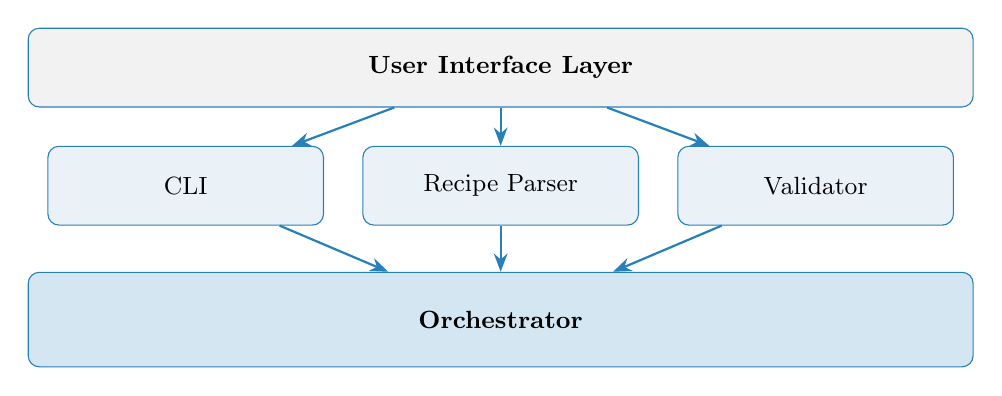
\begin{tikzpicture}[node distance=1.5cm and 2cm]
    % User layer
    \node[component, minimum width=12cm, fill=gray!10] (user) at (0, 5) {\textbf{User Interface Layer}};

    % Interface components
    \node[component, minimum width=3.5cm] (cli) at (-4, 3.5) {CLI};
    \node[component, minimum width=3.5cm] (recipe) at (0, 3.5) {Recipe Parser};
    \node[component, minimum width=3.5cm] (validator) at (4, 3.5) {Validator};

    % Orchestrator
    \node[component, minimum width=12cm, minimum height=1.2cm, fill=primary!20] (orch) at (0, 1.8) {\textbf{Orchestrator}};
    % Arrows
    \draw[arrow] (user) -- (cli);
    \draw[arrow] (user) -- (recipe);
    \draw[arrow] (user) -- (validator);
    \draw[arrow] (cli) -- (orch);
    \draw[arrow] (recipe) -- (orch);
    \draw[arrow] (validator) -- (orch);
\end{tikzpicture}
    \end{center}
\end{frame}

\begin{frame}{High-Level Architecture (Contd.)}
    \begin{center}
    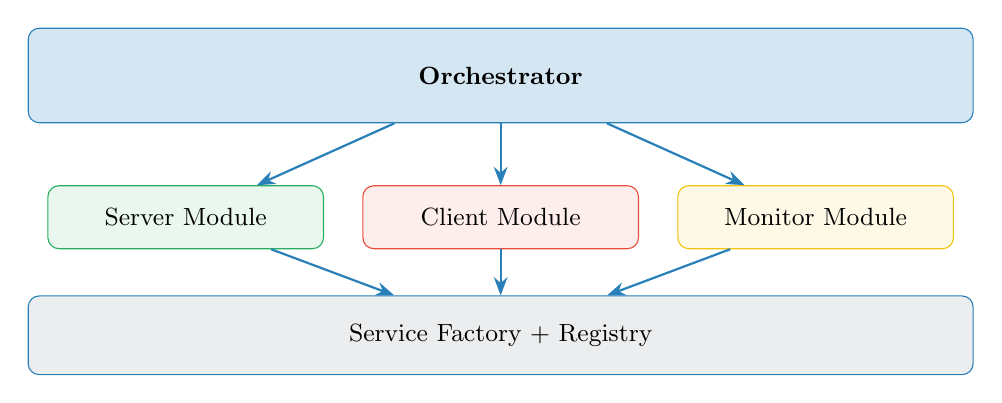
\begin{tikzpicture}[node distance=1.5cm and 2cm]
    % Orchestrator
    \node[component, minimum width=12cm, minimum height=1.2cm, fill=primary!20] (orch) at (0, 1.8) {\textbf{Orchestrator}};

    % Core modules
    \node[server, minimum width=3.5cm] (servers) at (-4, 0) {Server Module};
    \node[client, minimum width=3.5cm] (clients) at (0, 0) {Client Module};
    \node[monitor, minimum width=3.5cm] (monitors) at (4, 0) {Monitor Module};

    % Service Factory
    \node[component, minimum width=12cm, fill=secondary!10] (factory) at (0, -1.5) {Service Factory + Registry};

    % Arrows
    \draw[arrow] (orch) -- (servers);
    \draw[arrow] (orch) -- (clients);
    \draw[arrow] (orch) -- (monitors);
    \draw[arrow] (servers) -- (factory);
    \draw[arrow] (clients) -- (factory);
    \draw[arrow] (monitors) -- (factory);
\end{tikzpicture}
    \end{center}
\end{frame}

\begin{frame}{High-Level Architecture (Contd.)}
    \begin{center}
    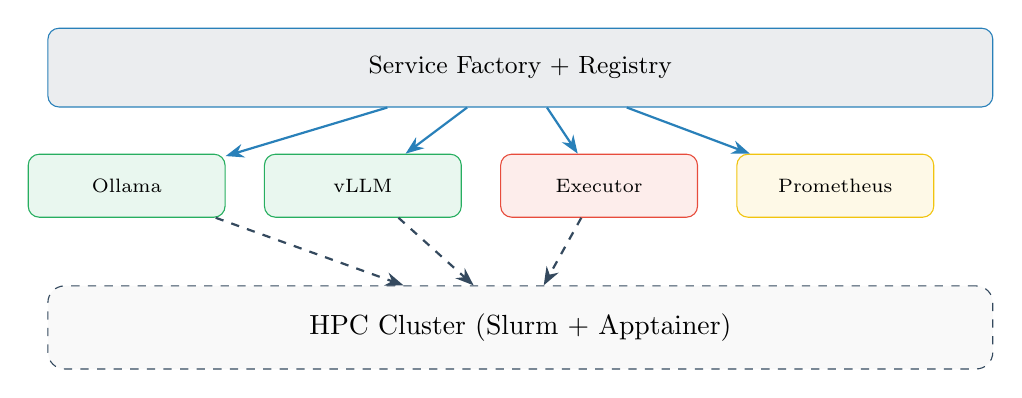
\begin{tikzpicture}[node distance=1.5cm and 2cm]
    % Service Factory
    \node[component, minimum width=12cm, fill=secondary!10] (factory) at (0, -1.5) {Service Factory + Registry};

    % Implementations
    \node[server, minimum width=2.5cm, font=\scriptsize] (ollama) at (-5, -3) {Ollama};
    \node[server, minimum width=2.5cm, font=\scriptsize] (vllm) at (-2, -3) {vLLM};
    \node[client, minimum width=2.5cm, font=\scriptsize] (exec1) at (1, -3) {Executor};
    \node[monitor, minimum width=2.5cm, font=\scriptsize] (prom) at (4, -3) {Prometheus};

    % Cluster layer
    \node[container, minimum width=12cm, minimum height=1cm, fill=gray!5] (cluster) at (0, -4.8) {HPC Cluster (Slurm + Apptainer)};

    % Arrows
    \draw[arrow] (factory) -- (ollama);
    \draw[arrow] (factory) -- (vllm);
    \draw[arrow] (factory) -- (exec1);
    \draw[arrow] (factory) -- (prom);
    \draw[dashedarrow] (ollama) -- (cluster);
    \draw[dashedarrow] (vllm) -- (cluster);
    \draw[dashedarrow] (exec1) -- (cluster);
\end{tikzpicture}
    \end{center}
\end{frame}


\begin{frame}{Six-Phase Execution Model}
    \begin{center}
    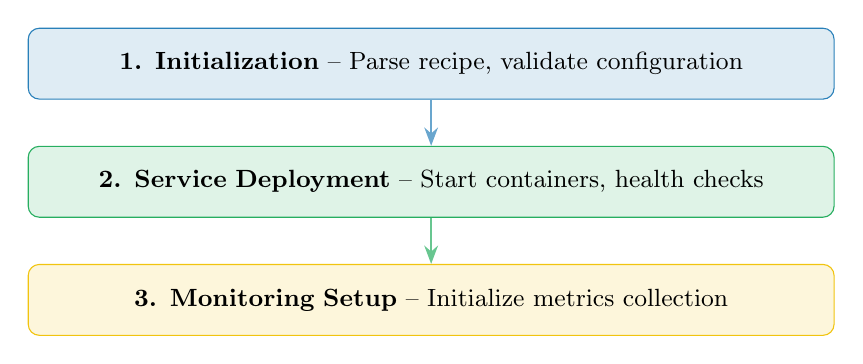
\begin{tikzpicture}[node distance=3cm]
        % Phase boxes with gradient-like effect
        \node[component, text width=10cm, minimum height=0.9cm, fill=primary!15] (p1) at (0, 0) {\textbf{1. Initialization} -- Parse recipe, validate configuration};
        \node[component, text width=10cm, minimum height=0.9cm, fill=success!15, draw=success] (p2) at (0, -1.5) {\textbf{2. Service Deployment} -- Start containers, health checks};
        \node[component, text width=10cm, minimum height=0.9cm, fill=warning!15, draw=warning] (p3) at (0, -3) {\textbf{3. Monitoring Setup} -- Initialize metrics collection};

        % Arrows between phases
        \draw[arrow, primary!70] (p1.south) -- (p2.north);
        \draw[arrow, success!70] (p2.south) -- (p3.north);
    \end{tikzpicture}
    \end{center}
\end{frame}

\begin{frame}{Six-Phase Execution Model (Contd.)}
    \begin{center}
    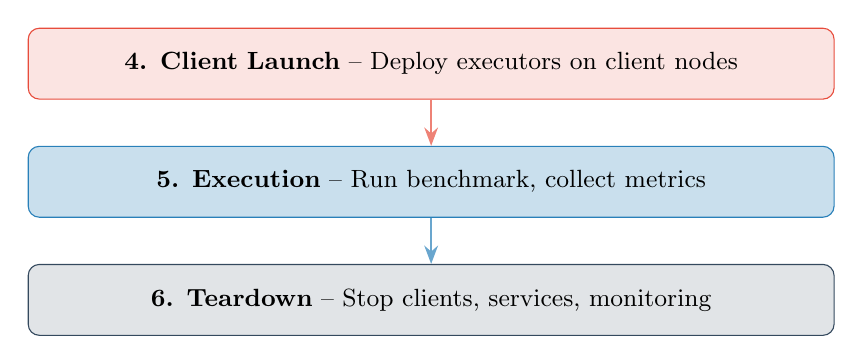
\begin{tikzpicture}[node distance=3cm]
        % Phase boxes with gradient-like effect
        \node[component, text width=10cm, minimum height=0.9cm, fill=accent!15, draw=accent] (p4) at (0, 0) {\textbf{4. Client Launch} -- Deploy executors on client nodes};
        \node[component, text width=10cm, minimum height=0.9cm, fill=primary!25] (p5) at (0, -1.5) {\textbf{5. Execution} -- Run benchmark, collect metrics};
        \node[component, text width=10cm, minimum height=0.9cm, fill=secondary!15, draw=secondary] (p6) at (0, -3) {\textbf{6. Teardown} -- Stop clients, services, monitoring};

        % Arrows between phases
        \draw[arrow, accent!70] (p4.south) -- (p5.north);
        \draw[arrow, primary!70] (p5.south) -- (p6.north);
    \end{tikzpicture}
    \end{center}
\end{frame}

\begin{frame}{Control Plane Communication}
    \begin{center}
    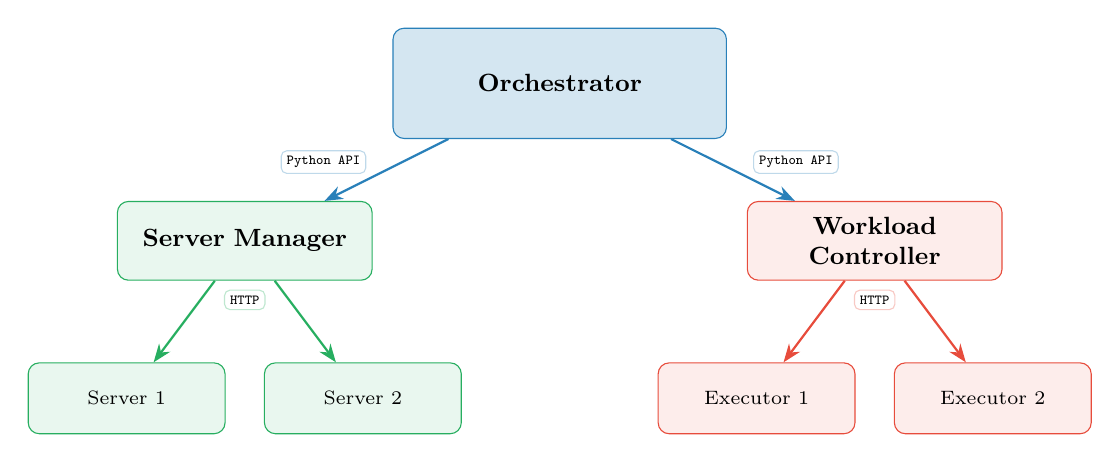
\begin{tikzpicture}[node distance=1cm]
        % Orchestrator
        \node[component, text width=4cm, minimum height=1.4cm, fill=primary!20] (orch) at (0, 3.5) {\textbf{Orchestrator}};

        % Server Manager
        \node[server, text width=3cm, minimum height=1cm] (sm) at (-4, 1.5) {\textbf{Server Manager}};

        % Workload Controller
        \node[client, text width=3cm, minimum height=1cm] (wc) at (4, 1.5) {\textbf{Workload Controller}};

        % Server nodes
        \node[server, text width=2.2cm, minimum height=0.9cm, font=\scriptsize] (s1) at (-5.5, -0.5) {Server 1};
        \node[server, text width=2.2cm, minimum height=0.9cm, font=\scriptsize] (s2) at (-2.5, -0.5) {Server 2};

        % Client executors
        \node[client, text width=2.2cm, minimum height=0.9cm, font=\scriptsize] (e1) at (2.5, -0.5) {Executor 1};
        \node[client, text width=2.2cm, minimum height=0.9cm, font=\scriptsize] (e2) at (5.5, -0.5) {Executor 2};

        % Protocol labels with boxes
        \node[fill=white, draw=primary!30, rounded corners=2pt, font=\tiny\ttfamily, inner sep=2pt] at (-3, 2.5) {Python API};
        \node[fill=white, draw=primary!30, rounded corners=2pt, font=\tiny\ttfamily, inner sep=2pt] at (3, 2.5) {Python API};
        \node[fill=white, draw=success!30, rounded corners=2pt, font=\tiny\ttfamily, inner sep=2pt] at (-4, 0.75) {HTTP};
        \node[fill=white, draw=accent!30, rounded corners=2pt, font=\tiny\ttfamily, inner sep=2pt] at (4, 0.75) {HTTP};

        % Arrows
        \draw[arrow] (orch) -- (sm);
        \draw[arrow] (orch) -- (wc);
        \draw[arrow, success] (sm) -- (s1);
        \draw[arrow, success] (sm) -- (s2);
        \draw[arrow, accent] (wc) -- (e1);
        \draw[arrow, accent] (wc) -- (e2);
    \end{tikzpicture}
    \end{center}
\end{frame}

\begin{frame}{Design Patterns}
    \begin{columns}[T]
        \begin{column}{0.48\textwidth}
            \begin{center}
            \textbf{\textcolor{primary}{Factory Pattern}}
            \end{center}
            \vspace{0.2cm}
            \begin{center}
            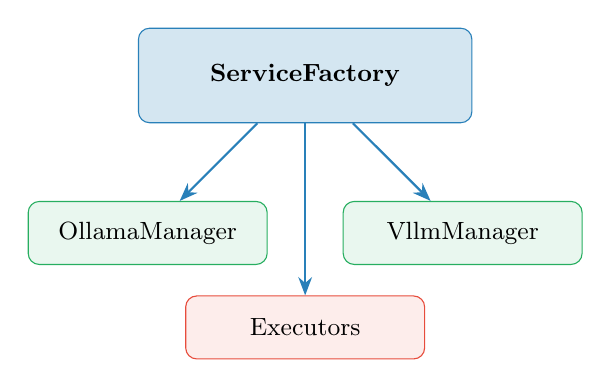
\begin{tikzpicture}[]
                \node[component, text width=4cm, minimum height=1.2cm, fill=primary!20] (factory) at (0, 2) {\textbf{ServiceFactory}};
                \node[server, text width=2.8cm] (ollama) at (-2, 0) {OllamaManager};
                \node[server, text width=2.8cm] (vllm) at (2, 0) {VllmManager};
                \node[client, text width=2.8cm] (exec) at (0, -1.2) {Executors};
                \draw[arrow] (factory) -- (ollama);
                \draw[arrow] (factory) -- (vllm);
                \draw[arrow] (factory) -- (exec);
            \end{tikzpicture}
            \end{center}
        \end{column}

        \begin{column}{0.48\textwidth}
            \begin{center}
            \textbf{\textcolor{primary}{Template Method Pattern}}
            \end{center}
            \vspace{0.2cm}
            \begin{center}
            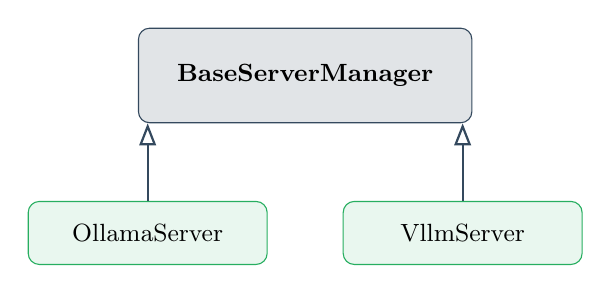
\begin{tikzpicture}[]
                \node[component, text width=4cm, minimum height=1.2cm, fill=secondary!15, draw=secondary] (base) at (0, 2) {\textbf{BaseServerManager}};
                \node[server, text width=2.8cm] (ollama) at (-2, 0) {OllamaServer};
                \node[server, text width=2.8cm] (vllm) at (2, 0) {VllmServer};
                % Inheritance arrows (hollow)
                \draw[thick, -{Triangle[open, length=8pt, width=6pt]}, secondary] (ollama.north) -- (base.south -| ollama);
                \draw[thick, -{Triangle[open, length=8pt, width=6pt]}, secondary] (vllm.north) -- (base.south -| vllm);
            \end{tikzpicture}
            \end{center}
        \end{column}
    \end{columns}
\end{frame}

% ============================================================================
\section{Infrastructure}
% ============================================================================

\begin{frame}{Recipe Configuration System}
    \begin{center}
    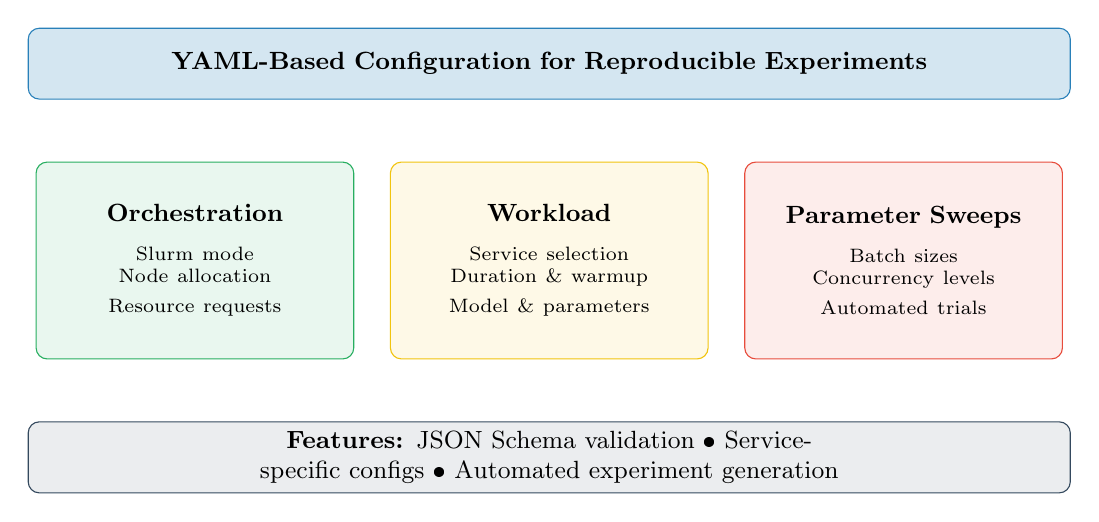
\begin{tikzpicture}
        % Title box
        \node[component, text width=13cm, minimum height=0.9cm, fill=primary!20] at (0, 3) {
            \textbf{YAML-Based Configuration for Reproducible Experiments}
        };

        % Three key aspects
        \node[component, text width=3.8cm, minimum height=2.5cm, fill=success!10, draw=success] at (-4.5, 0.5) {
            \textbf{Orchestration}\\[6pt]
            {\scriptsize Slurm mode\\
            Node allocation\\
            Resource requests}
        };

        \node[component, text width=3.8cm, minimum height=2.5cm, fill=warning!10, draw=warning] at (0, 0.5) {
            \textbf{Workload}\\[6pt]
            {\scriptsize Service selection\\
            Duration \& warmup\\
            Model \& parameters}
        };

        \node[component, text width=3.8cm, minimum height=2.5cm, fill=accent!10, draw=accent] at (4.5, 0.5) {
            \textbf{Parameter Sweeps}\\[6pt]
            {\scriptsize Batch sizes\\
            Concurrency levels\\
            Automated trials}
        };

        % Bottom feature
        \node[component, text width=13cm, minimum height=0.8cm, fill=secondary!10, draw=secondary] at (0, -2) {
            \textbf{Features:} JSON Schema validation \textbullet{} Service-specific configs \textbullet{} Automated experiment generation
        };
    \end{tikzpicture}
    \end{center}
\end{frame}

\begin{frame}{Recipe Validation}
    \begin{placeholder}{Laura's Section}
        \begin{itemize}
            \item JSON Schema validation implementation
            \item Validation rules and error messages
            \item Custom validators for service-specific configs
            \item Schema versioning support
            \item Interactive validation mode
        \end{itemize}
    \end{placeholder}
\end{frame}

\begin{frame}{Slurm Integration}
    	\textbf{Recipe-Driven SLURM Job Setup}
    \vspace{0.3cm}
    \begin{itemize}
        \item The recipe is parsed to determine the required services, replicas, and node allocation.
        \item A SLURM job is created according to the configuration, reserving the correct number of nodes and resources.
        \item On each node, the appropriate Apptainer container is spawned:
        \begin{itemize}
            \item Server nodes: start service Apptainer (e.g., Ollama)
            \item Client nodes: start Python Apptainer for workload execution
            \item Orchestrator/monitoring/logging node: start orchestrator and monitoring services
        \end{itemize}
    \end{itemize}
\end{frame}

\begin{frame}{Slurm Integration (Contd.)}
    \begin{itemize}
        \item The orchestrator coordinates all components, waits for services to be online, and provides clients with service type, URLs, and ports.
        \item Clients use multithreaded service worker implementations to send requests to the services.
        \item Only the orchestrator is stateful; all other components are stateless and report to the orchestrator.
    \end{itemize}
\end{frame}

% ============================================================================
\section{SLURM Job Lifecycle: Example}
% ============================================================================

\begin{frame}{Step 1: Recipe Configuration}
    	\textbf{User provides a YAML recipe:}
    \begin{itemize}
        \item 2 server nodes (Ollama)
        \item 2 client nodes (100 clients per node)
        \item 1 node for orchestrator/monitoring/logging
    \end{itemize}
    \vspace{0.2cm}
    	\textbf{Goal:} Benchmark Ollama service with 200 concurrent clients.
\end{frame}

\begin{frame}{Step 2: SLURM Job Creation}
    \begin{itemize}
        \item The system parses the recipe and generates a SLURM job script.
        \item \textbf{Resources reserved:} 5 nodes (2 server, 2 client, 1 orchestrator/monitoring/logging)
        \item Each node is assigned a specific role based on the recipe.
    \end{itemize}
\end{frame}

\begin{frame}{Step 3: Node Setup}
    \begin{itemize}
        \item \textbf{Server nodes:} Start Ollama Apptainer service
        \item \textbf{Client nodes:} Start Python Apptainer, each running 100 client threads
        \item \textbf{Orchestrator/monitoring/logging node:} Start orchestrator, monitoring, and logging services
    \end{itemize}
\end{frame}

\begin{frame}{Step 4: Orchestrator Actions}
    \begin{itemize}
        \item Waits for all services to be online
        \item Discovers service types, URLs, and ports
        \item Provides clients with connection details
        \item Coordinates the experiment, tracks state, and aggregates results
    \end{itemize}
    	\textbf{Note:} Orchestrator is the only stateful component; all others are stateless.
\end{frame}

\begin{frame}{Step 5: Client Behavior}
    \begin{itemize}
        \item Each client thread uses the provided service worker implementation
        \item Sends requests to the correct service endpoint (Ollama)
        \item Collects metrics and reports results to the orchestrator
    \end{itemize}
    	\textbf{Result:} Scalable, reproducible benchmarking with full orchestration and monitoring.
\end{frame}

\begin{frame}{Distributed vLLM with Ray}
    \begin{itemize}
        \item \textbf{Ray-based vLLM (Distributed):} Uses a master/worker architecture (Ray Head + Ray Workers).
        \item \textbf{Single Endpoint:} All distributed workers are managed by the Ray Head node, exposing a single API endpoint for clients.
        \item \textbf{Tensor Parallelism:} Multiple GPUs across several nodes are coordinated for high-throughput inference.
        \item \textbf{Contrast with Ollama/Non-Distributed vLLM:}
        \begin{itemize}
            \item \textbf{Ollama:} Each server node runs a fully separated service instance, each with its own endpoint.
            \item \textbf{vLLM (non-distributed):} Single-node, single service, single endpoint.
            \item \textbf{Ray Distributed:} Multiple worker nodes are managed under one master, with all services accessible via a unique, unified endpoint (more realistic for production).
        \end{itemize}
        \item \textbf{Implication:} Clients connect to one endpoint, and Ray transparently distributes requests across all available GPUs/nodes.
    \end{itemize}
\end{frame}


% ============================================================================
\section{Monitoring}
% ============================================================================

\begin{frame}{Monitoring Architecture}
    \textbf{Prometheus + Grafana Stack}
    \vspace{0.3cm}
    \begin{itemize}
        \item \textbf{Executors:} Expose metrics via HTTP endpoints (\texttt{/metrics/prometheus})
        \item \textbf{Prometheus:} Time-series database, scrapes metrics periodically
        \item \textbf{Grafana:} Visualization dashboards with custom panels
        \item \textbf{Deployment:} Docker Compose for easy setup (local + HPC)
    \end{itemize}
    
    \vspace{0.3cm}
    \textbf{Key Metrics Collected:}
    \begin{itemize}
        \item Request count, errors, success rate
        \item Latency (average, P50, P90, P99)
        \item Throughput (requests per second)
        \item System resources (CPU, memory, active threads)
    \end{itemize}
\end{frame}

\begin{frame}{MeluXina Integration}
    \textbf{Challenge:} Compute nodes not directly accessible from outside
    
    \vspace{0.3cm}
    \textbf{Solution:} Automated SSH tunneling
    \begin{itemize}
        \item \texttt{setup\_monitoring.sh} script identifies Slurm node allocation
        \item Establishes SSH tunnels from login node to each executor endpoint
        \item Makes metrics accessible to Prometheus
        \item Handles cleanup when job completes
    \end{itemize}
    
    \vspace{0.3cm}
    \textbf{Dashboards:}
    \begin{itemize}
        \item \textbf{Ollama Dashboard:} API performance, response times
        \item \textbf{vLLM Dashboard:} API endpoints, cluster performance
    \end{itemize}
    
    \vspace{0.2cm}
    \textit{Metrics collected after benchmark completion for analysis}
\end{frame}

% ============================================================================
\section{Logging System}
% ============================================================================

\begin{frame}{Logging Architecture}
    \begin{placeholder}{Giulia's Section}
        \textbf{Overall Design:}
        \begin{itemize}
            \item Log sources and destinations
            \item Aggregation strategy for distributed logs
        \end{itemize}

        \vspace{0.3cm}
        \textbf{BaseLogCollector:}
        \begin{itemize}
            \item Abstract interface design
            \item LogSource dataclass
        \end{itemize}

        \vspace{0.3cm}
        \textbf{TailerLogCollector:}
        \begin{itemize}
            \item File tailing implementation
            \item Remote node log collection
        \end{itemize}
    \end{placeholder}
\end{frame}

\begin{frame}{Log Categories and Storage}
    \begin{placeholder}{Giulia's Section}
        \textbf{Log Categories:}
        \begin{itemize}
            \item Application logs
            \item System logs (Slurm)
            \item Benchmark logs
            \item Infrastructure logs
        \end{itemize}

        \vspace{0.3cm}
        \textbf{Log Format:}
        \begin{itemize}
            \item Structured logging (JSON)
            \item Timestamps and correlation IDs
            \item Storage organization
            \item Retention policies
        \end{itemize}
    \end{placeholder}
\end{frame}

% ============================================================================
\section{Benchmarking}
% ============================================================================

\begin{frame}{Performance Analysis}
    \begin{placeholder}{Laura's Benchmarking Results}
        \textbf{Bottleneck Analysis:}
        \begin{itemize}
            \item Latency breakdown for LLM inference
            \item GPU compute vs memory transfer
            \item Network overhead measurements
        \end{itemize}

        \vspace{0.3cm}
        \textbf{Scaling Analysis:}
        \begin{itemize}
            \item Single-node vs multi-node performance
            \item Strong/weak scaling efficiency
        \end{itemize}

        \vspace{0.3cm}
        \textit{Include benchmark charts and graphs here}
    \end{placeholder}
\end{frame}

% ============================================================================
\section{Division of Work}
% ============================================================================

\begin{frame}{Alberto Finardi}
    	\textbf{System Architect \& Core Implementation}
    \vspace{0.3cm}
    \begin{itemize}
        \item \textbf{Infrastructure:} Core architecture, Factory pattern, Service registry
        \item \textbf{Server Managers:} Ollama, vLLM, Ray orchestration
        \item \textbf{Workload System:} Controllers, Executors, Benchmarking
        \item \textbf{Logging:} Base information logging system
        \item \textbf{Integration:} CLI interface, Slurm orchestration, Documentation
    \end{itemize}
\end{frame}

\begin{frame}{Giovanni La Gioia}
    	\textbf{Monitoring \& Observability}
    \vspace{0.3cm}
    \begin{itemize}
        \item \textbf{Prometheus:} Configuration, Metric collection, Scraping setup
        \item \textbf{Grafana:} Dashboard design, Visualization
    \end{itemize}
\end{frame}

\begin{frame}{Laura Paxton}
    	\textbf{Recipe Validation \& Benchmark Execution}
    \vspace{0.3cm}
    \begin{itemize}
        \item \textbf{Validation:} JSON Schema, Error formatting
        \item \textbf{Benchmarking:} Tested Ollama execution, vLLM execution, Parameter sweeps, Result analysis
    \end{itemize}
\end{frame}

\begin{frame}{Giulia Lionetti}
    	\textbf{Logging System Architecture}
    \vspace{0.3cm}
    \begin{itemize}
        \item \textbf{Architecture:} BaseLogCollector, Abstract interfaces, LogSource design, Strategy pattern
        \item \textbf{Implementation:} TailerLogCollector, Remote collection, Structured JSON, Aggregation
    \end{itemize}
\end{frame}

\begin{frame}{Questions?}
    \begin{center}
        {\Huge \textbf{Thank You!}}

        \vspace{0.5cm}
        {\Large \textbf{Questions?}}

        \vspace{0.5cm}
        {\small \texttt{hpc-benchmark-toolkit} | MeluXina HPC Cluster}
    \end{center}
\end{frame}

\end{document}
